 
\begin{figure}[t]
    \centering
    \subfigure[ svhn--ResNeXt, $\langle\log\Vert\cdot\Vert_{F}\rangle$ ]{
        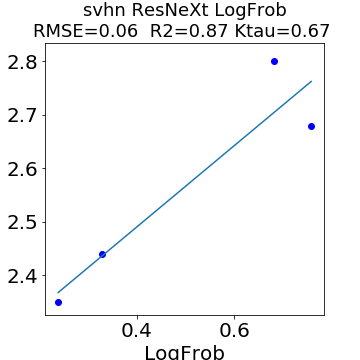
\includegraphics[width=3.7cm]{img/omsr_svhn_ResNeXt_lognorm}
        \label{fig:summary_regressions_I_01}
    }
    \subfigure[ svhn--ResNeXt, $\langle\log\Vert\cdot\Vert_{\infty}\rangle$ ]{
        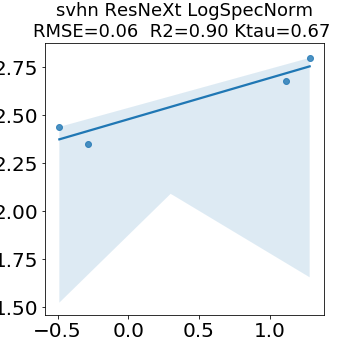
\includegraphics[width=3.7cm]{img/omsr_svhn_ResNeXt_spectralnormlog}
        \label{fig:summary_regressions_I_02}
    }
    \subfigure[ svhn--ResNeXt, $\hat{\alpha}$ ]{
        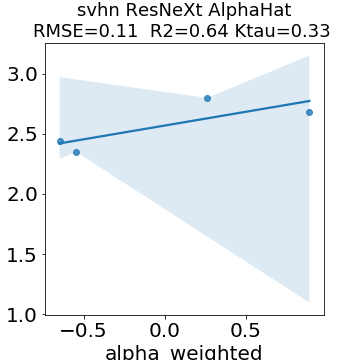
\includegraphics[width=3.7cm]{img/omsr_svhn_ResNeXt_alpha_weighted}
        \label{fig:summary_regressions_I_03}
    }
    \subfigure[ svhn--ResNeXt, $\langle\log\Vert\cdot\Vert^{\alpha}_{\alpha}\rangle$ ]{
        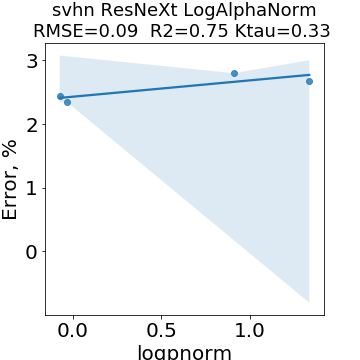
\includegraphics[width=3.7cm]{img/omsr_svhn_ResNeXt_logpnorm}
        \label{fig:summary_regressions_I_04}
    }
    \subfigure[ cub-200-2011--ResNet, $\langle\log\Vert\cdot\Vert_{F}\rangle$ ]{
        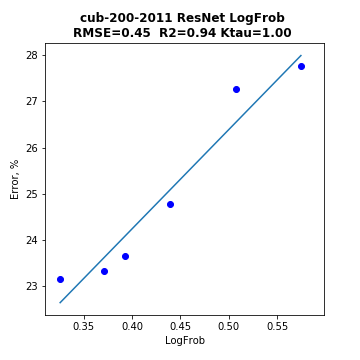
\includegraphics[width=3.7cm]{img/omsr_cub_200_2011_ResNet_lognorm}
        \label{fig:summary_regressions_I_05}
    }
    \subfigure[ cub-200-2011--ResNet, $\langle\log\Vert\cdot\Vert_{\infty}\rangle$ ]{
        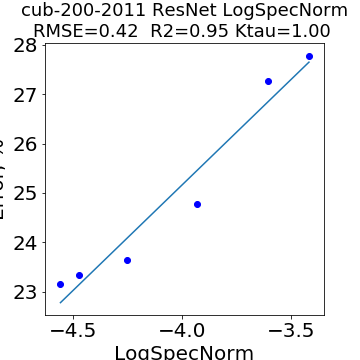
\includegraphics[width=3.7cm]{img/omsr_cub_200_2011_ResNet_spectralnormlog}
        \label{fig:summary_regressions_I_06}
    }
    \subfigure[ cub-200-2011--ResNet, $\hat{\alpha}$ ]{
        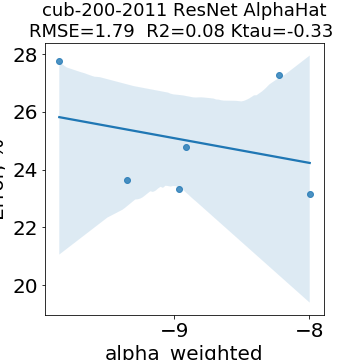
\includegraphics[width=3.7cm]{img/omsr_cub_200_2011_ResNet_alpha_weighted}
        \label{fig:summary_regressions_I_07}
    }
    \subfigure[ cub-200-2011--ResNet, $\langle\log\Vert\cdot\Vert^{\alpha}_{\alpha}\rangle$ ]{
        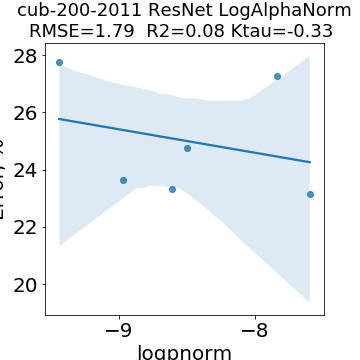
\includegraphics[width=3.7cm]{img/omsr_cub_200_2011_ResNet_logpnorm}
        \label{fig:summary_regressions_I_08}
    }
    \subfigure[ cub-200-2011--SENet, $\langle\log\Vert\cdot\Vert_{F}\rangle$ ]{
        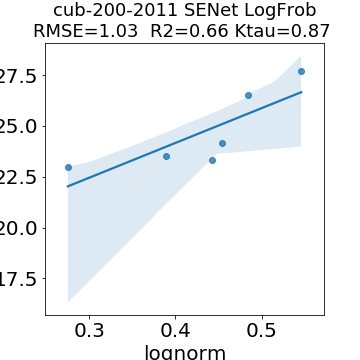
\includegraphics[width=3.7cm]{img/omsr_cub_200_2011_SENet_lognorm}
        \label{fig:summary_regressions_I_09}
    }
    \subfigure[ cub-200-2011--SENet, $\langle\log\Vert\cdot\Vert_{\infty}\rangle$ ]{
        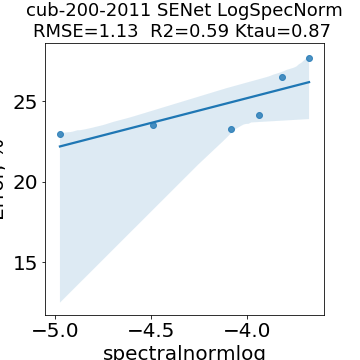
\includegraphics[width=3.7cm]{img/omsr_cub_200_2011_SENet_spectralnormlog}
        \label{fig:summary_regressions_I_10}
    }
    \subfigure[ cub-200-2011--SENet, $\hat{\alpha}$ ]{
        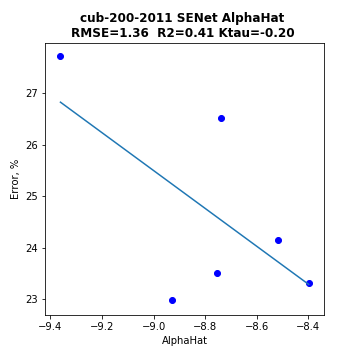
\includegraphics[width=3.7cm]{img/omsr_cub_200_2011_SENet_alpha_weighted}
        \label{fig:summary_regressions_I_11}
    }
    \subfigure[ cub-200-2011--SENet, $\langle\log\Vert\cdot\Vert^{\alpha}_{\alpha}\rangle$ ]{
        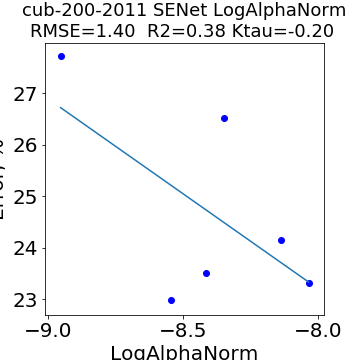
\includegraphics[width=3.7cm]{img/omsr_cub_200_2011_SENet_logpnorm}
        \label{fig:summary_regressions_I_12}
    }
    \caption{Regression plots for model-dataset pairs, based on data from Table~\ref{table:RMSEresults}, Table~\ref{table:R2results}, and Table~\ref{table:Ktauresults}.
             Each row corresponds to a different dataset-model pair:
             svhn--ResNeXt;
             cub-200-2011--ResNet;
             and
             cub-200-2011--SENet;
             repsectively.
             Each column corresponds to a different metric:
             $\langle\log\Vert\cdot\Vert_{F}\rangle$; 
             $\langle\log\Vert\cdot\Vert_{\infty}\rangle$; 
             $\hat{\alpha}$; 
             and
             $\langle\log\Vert\cdot\Vert^{\alpha}_{\alpha}\rangle$;
             repsectively.
            }
    \label{fig:summary_regressions_I}
\end{figure}

 







